\documentclass[tikz]{standalone}
\standaloneconfig{border=1cm} 
\usepackage[utf8]{inputenc}

\usetikzlibrary{calc}

\title{Weight Sharing in CNNs}
\author{James Allingham}
\date{April 2019}

\begin{document}

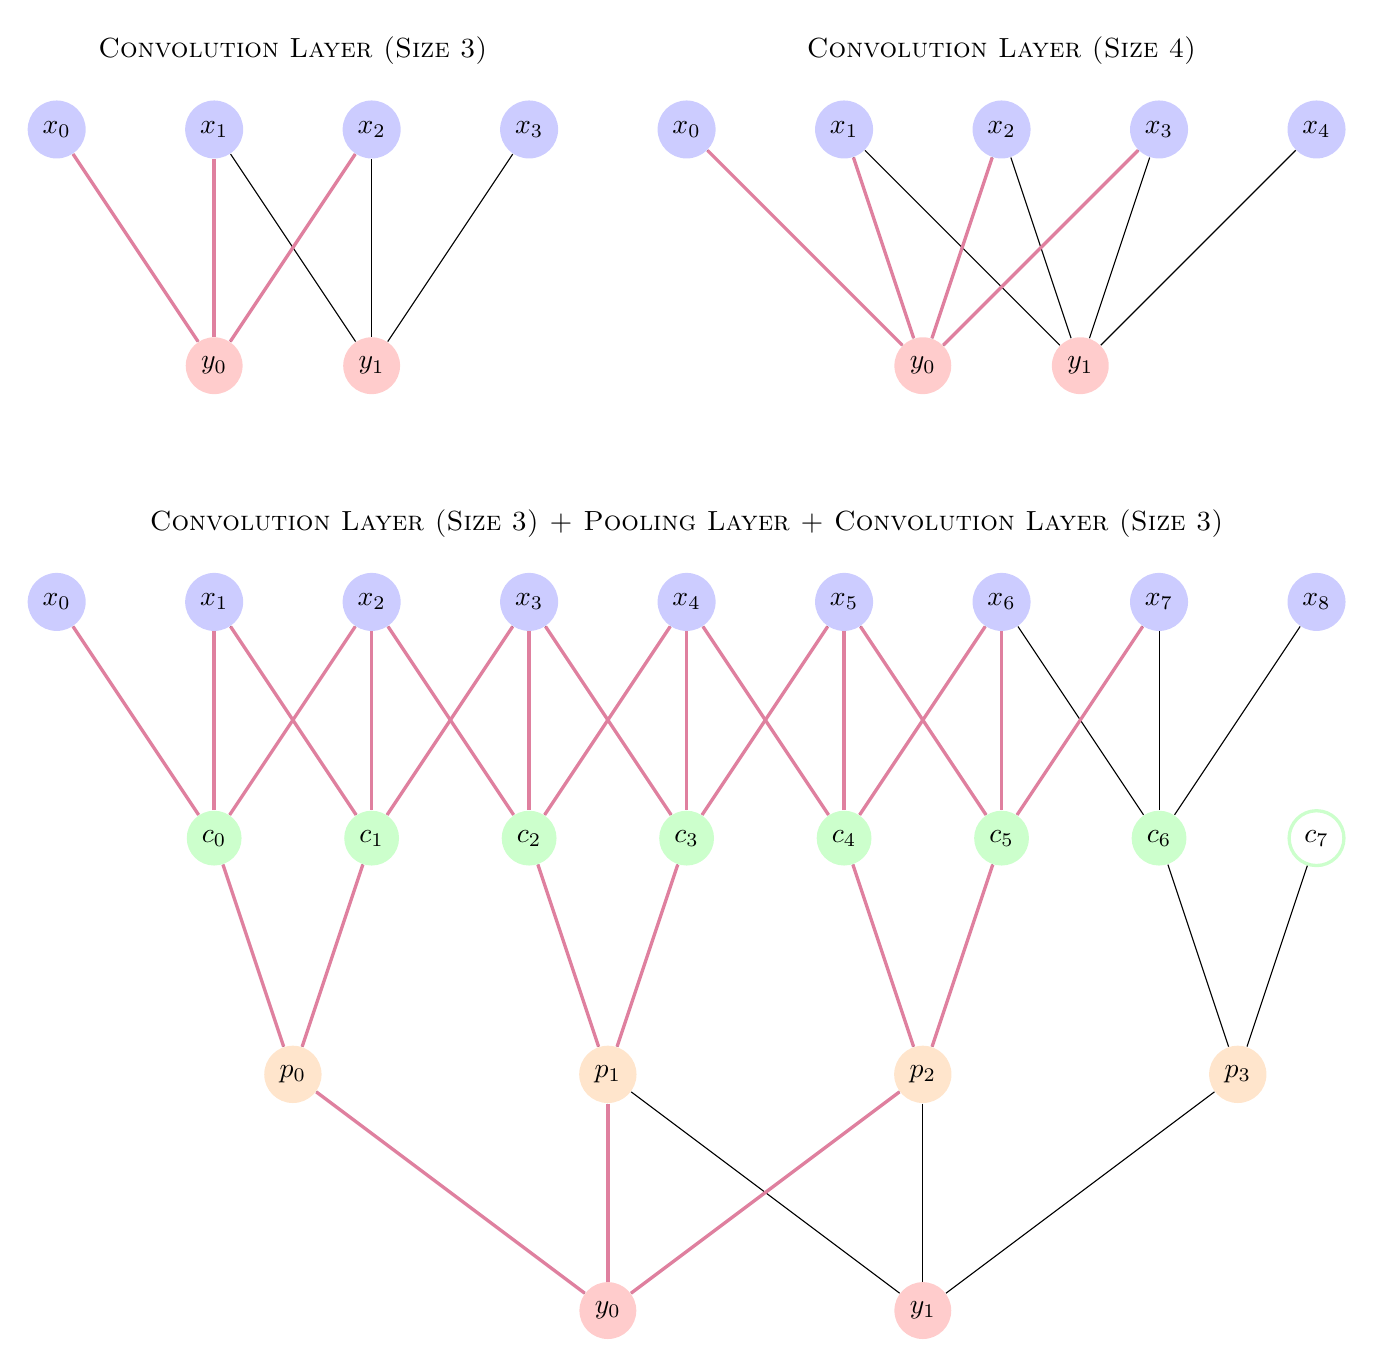
\begin{tikzpicture}
    % \draw[help lines](0,-15) grid (20,5);    
    
    % Convolution Layer (Size 3):
    \node[] at (3,4) {\textsc{Convolution Layer (Size 3)}};
    
    % input nodes
    \foreach \z in {0,1,...,3} {
        \node[circle, fill=blue!20, label={}, minimum size=0.5cm] (z\z) at ($2*(\z,0) + (0,3)$) {$x_{\z}$};
    }
    
    % output nodes and edges
    \foreach \y in {0,1,...,1} {
        \node[circle, fill=red!20, label={}, minimum size=0.5cm] (y\y) at ($2*(\y,0) + (2,0)$) {$y_{\y}$};
        \pgfmathsetmacro{\prev}{\y};
        \pgfmathtruncatemacro{\cur}{\y + 1};
        \pgfmathtruncatemacro{\next}{\y + 2};
        \path[draw=black] (z\prev) edge[-] (y\y);
        \path[draw=black] (z\cur) edge[-]  (y\y);
        \path[draw=black] (z\next) edge[-] (y\y);
    }
    
    % Highlight receptive field for y0
    \path[draw=purple!50, very thick] (z0) edge[-] (y0);
    \path[draw=purple!50, very thick] (z1) edge[-] (y0);
    \path[draw=purple!50, very thick] (z2) edge[-] (y0);
    
    % Convolution Layer (Size 4):
    \node[] at (12,4) {\textsc{Convolution Layer (Size 4)}};
    
    % input nodes
    \foreach \z in {0,1,...,4} {
        \node[circle, fill=blue!20, label={}, minimum size=0.5cm] (z\z) at ($2*(\z,0) + (0,3) + (8,0)$) {$x_{\z}$};
    }
    
    % output nodes and edges
    \foreach \y in {0,1,...,1} {
        \node[circle, fill=red!20, label={}, minimum size=0.5cm] (y\y) at ($2*(\y,0) + (3,0)  + (8,0)$) {$y_{\y}$};
        \pgfmathsetmacro{\prev}{\y};
        \pgfmathtruncatemacro{\cur}{\y + 1};
        \pgfmathtruncatemacro{\next}{\y + 2};
        \pgfmathtruncatemacro{\nextnext}{\y + 3};
        \path[draw=black] (z\prev) edge[-] (y\y);
        \path[draw=black] (z\cur) edge[-]  (y\y);
        \path[draw=black] (z\next) edge[-] (y\y);
        \path[draw=black] (z\nextnext) edge[-] (y\y);
    }
    
    % Highlight receptive field for y0
    \path[draw=purple!50, very thick] (z0) edge[-] (y0);
    \path[draw=purple!50, very thick] (z1) edge[-] (y0);
    \path[draw=purple!50, very thick] (z2) edge[-] (y0);
    \path[draw=purple!50, very thick] (z3) edge[-] (y0);
    
    % Convolution Layer (Size 3) * 2 + pooling :
    \node[] at (8,-2) {\textsc{Convolution Layer (Size 3) + Pooling Layer + Convolution Layer (Size 3)}};
    
    % input nodes
    \foreach \z in {0,1,...,8} {
        \node[circle, fill=blue!20, label={}, minimum size=0.5cm] (z\z) at ($2*(\z,0) + (0,9) + (0,-12)$) {$x_{\z}$};
    }
    
    % hidden nodes and edges
    \foreach \c in {0,1,...,6} {
        \node[circle, fill=green!20, label={}, minimum size=0.5cm] (c\c) at ($2*(\c,0) + (2,6)  + (0,-12)$) {$c_{\c}$};
        \pgfmathsetmacro{\prev}{\c};
        \pgfmathtruncatemacro{\cur}{\c + 1};
        \pgfmathtruncatemacro{\next}{\c + 2};
        \path[draw=black] (z\prev) edge[-] (c\c);
        \path[draw=black] (z\cur) edge[-]  (c\c);
        \path[draw=black] (z\next) edge[-] (c\c);
    }
    
    \node[circle, draw=green!20, label={}, minimum size=0.5cm, very thick] (c7) at ($2*(7,0) + (2,6)  + (0,-12)$) {$c_{7}$};
    
    % pooling nodes and edges
    \foreach \p in {0,1,...,3} {
        \node[circle, fill=orange!20, label={}, minimum size=0.5cm] (p\p) at ($3*(\p,0) + (3,3) + (\p,0)  + (0,-12)$) {$p_{\p}$};
        \pgfmathtruncatemacro{\prev}{2 * \p};
        \pgfmathtruncatemacro{\cur}{2 * \p + 1};
        \path[draw=black] (c\prev) edge[-] (p\p);
        \path[draw=black] (c\cur) edge[-]  (p\p);
    }
    
    % output nodes and edges
    \foreach \y in {0,1,...,1} {
        \node[circle, fill=red!20, label={}, minimum size=0.5cm] (y\y) at ($2*(\y,0) + (7,0) + 2*(\y,0)  + (0,-12)$) {$y_{\y}$};
        \pgfmathsetmacro{\prev}{\y};
        \pgfmathtruncatemacro{\cur}{\y + 1};
        \pgfmathtruncatemacro{\next}{\y + 2};
        \path[draw=black] (p\prev) edge[-] (y\y);
        \path[draw=black] (p\cur) edge[-]  (y\y);
        \path[draw=black] (p\next) edge[-] (y\y);
    }
    
    % Highlight receptive field for y0
    \path[draw=purple!50, very thick] (p0) edge[-] (y0);
    \path[draw=purple!50, very thick] (p1) edge[-] (y0);
    \path[draw=purple!50, very thick] (p2) edge[-] (y0);
    \path[draw=purple!50, very thick] (c0) edge[-] (p0);
    \path[draw=purple!50, very thick] (c1) edge[-] (p0);
    \path[draw=purple!50, very thick] (c2) edge[-] (p1);
    \path[draw=purple!50, very thick] (c3) edge[-] (p1);
    \path[draw=purple!50, very thick] (c4) edge[-] (p2);
    \path[draw=purple!50, very thick] (c5) edge[-] (p2);
    \path[draw=purple!50, very thick] (c0) edge[-] (z0);
    \path[draw=purple!50, very thick] (c0) edge[-] (z1);
    \path[draw=purple!50, very thick] (c0) edge[-] (z2);
    \path[draw=purple!50, very thick] (c1) edge[-] (z1);
    \path[draw=purple!50, very thick] (c1) edge[-] (z2);
    \path[draw=purple!50, very thick] (c1) edge[-] (z3);
    \path[draw=purple!50, very thick] (c2) edge[-] (z2);
    \path[draw=purple!50, very thick] (c2) edge[-] (z3);
    \path[draw=purple!50, very thick] (c2) edge[-] (z4);
    \path[draw=purple!50, very thick] (c3) edge[-] (z3);
    \path[draw=purple!50, very thick] (c3) edge[-] (z4);
    \path[draw=purple!50, very thick] (c3) edge[-] (z5);
    \path[draw=purple!50, very thick] (c4) edge[-] (z4);
    \path[draw=purple!50, very thick] (c4) edge[-] (z5);
    \path[draw=purple!50, very thick] (c4) edge[-] (z6);
    \path[draw=purple!50, very thick] (c5) edge[-] (z5);
    \path[draw=purple!50, very thick] (c5) edge[-] (z6);
    \path[draw=purple!50, very thick] (c5) edge[-] (z7);

\end{tikzpicture}

\end{document}
